\documentclass[a4paper, 12pt]{article}

%\usepackage{cmap}
\usepackage[T2A]{fontenc}
\usepackage[utf8]{inputenc}
\usepackage[english, russian]{babel}
\usepackage{graphicx}
\usepackage[top=1in, bottom=1in, left=3.2cm, right=2.6cm]{geometry}
\graphicspath{./}
\usepackage{biblatex}
\addbibresource{lib.bib}
\linespread{1.5}
\usepackage{ragged2e}
\justifying
\usepackage{listings}
\usepackage{color}


\begin{document}
	
\begin{titlepage}
	\fontsize{12pt}{12pt}\selectfont
	\begin{figure}[t!]
		\centering
		
\includegraphics[scale=0.8]{bmstu}
	\end{figure}
	
	\noindent\rule{15cm}{3pt}
	\newline\newline
	\noindent 
	ФАКУЛЬТЕТ 
	\underline{«Информатика и системы управления»} \newline\newline
	
	\noindent КАФЕДРА \underline{«Программное обеспечение ЭВМ и информационные технологии»}\newline\newline\newline\newline\newline
	
	\centering {\Large Отчет по лабораторной работе № 2}
	\vspace{1mm}
	
	\centering {\Large По курсу: "Функциональное и логическое программирование"
		\vspace{8mm}	
		
		\centering \bf Списки в Lisp. Использование стандартных функций.}
	\vspace{8mm}
	
	
	\begin{flushright}
		{\small	Студент:\\ Турсунов Жасурбек Рустамович \\ Группа: ИУ7-56Б
			\vspace{3mm}
			\\Преподователи: \\ Толпинская Наталья Борисовна \\ Строганов Юрий Владимирович}
	\end{flushright}
	
	\begin{center}
		\vfill
		Москва, \the\year
		~г.
	\end{center}
\end{titlepage}

\tableofcontents
\clearpage
\newpage

\textbf{Цель работы:} приобрести навыки использования списков и стандартных функций Lisp.
\\ \hspace*{5mm} \textbf{Задачи работы:} изучить способ использования списков для фиксации информации, внутреннее представление одноуровневых и структурированных списков, методы их обработки с использованием базовых функций Lisp.


\section*{Введение}
\addcontentsline{toc}{section}{Введение}

\hspace*{5mm} \textbf{Функция} в Лиспе есть однозначное отображение множества исходных данных на множество её значений. У функции может быть произвольно много аргументов, от нуля до любого конечного числа, но обязательно должно быть хотя бы одно значение.
\\ \textbf{Классификация функций}
\begin{enumerate}
	\item базовые функции - принимают фиксированное количество аргументов;
	\item формы - принимают не фиксированное количество аргументов или обрабатывают аргументы по разному;
	\item Функционалы (высших порядков) - использут другие функции в качестве аргументов или вырабатывают в качестве результатов. 
\end{enumerate}
 \hspace*{5mm} \textbf{CAR и CDR} являются базовыми функциями доступа к данным. CAR принимает точечную пару или пустой список в качестве аргумента и возвращает первый элемент или nil, соответственно. CDR принимает точечную пару или пустой список и возвращает список состоящий из всех элементов, кроме первого. Если в списке меньше 2 элементов, то возращается nil.
 \\ \hspace*{5mm} \textbf{LIST и CONS} являются функциями создания списков (cons - базовая, list - нет). Функция <<cons>> создает списочную ячейку и устанавливает два указателя на аргументы. Функция list принимает переменное число аргументов и возвращает список, элементы которого  - переданные в функцию аргументы.

\section*{Задание 2}
\addcontentsline{toc}{section}{Задание 2}
Используя только функции CAR и CDR, написать выражения, возвращающие следующие элементы списка:
\begin{enumerate}
	\item второй -> cadr('(1 2 3 4 5));
	\item третий -> caddr('(1 2 3 4 5));
	\item четвертый -> cadddr('(1 2 3 4 5)).
\end{enumerate}

\section*{Задание 3}
\addcontentsline{toc}{section}{Задание 3}
Что будет в результате вычисления выражений:
\begin{enumerate}
	\item (caadr '((blue cube) (red pyramid))) -> red;
	\item (cdar '((abc)(def)(ghi))) -> nil;
	\item (cadr '((abc)(def)(ghi))) -> def;
	\item (caddr '((abc)(def)(ghi))) -> ghi.
\end{enumerate}

\section*{Задание 4}
\addcontentsline{toc}{section}{Задание 4}
Напишите результат вычисления выражений:
\begin{enumerate}
	\item (list 'Fred 'and 'Wilma) -> (Fred and Wilma);
	\item (list 'Fred '(and Wilma)) -> (Fred (and Wilma));
	\item (cons Nil Nil) -> (Nil);
	\item (cons T Nil) -> (T);
	\item (cons Nil T) -> (Nil.T);
	\item (list Nil) -> (Nil);
	\item (cons '(T) Nil) -> ((T));
	\item (list '(one two) '(free temp)) -> ((one two) (free temp));
	\item (cons 'Fred '(and Wilma)) -> (Fred (and Wilma));
	\item (cons 'Fred '(Wilma)) -> (Fred Wilma);
	\item (list Nil Nil) -> (Nil Nil);
	\item (list T Nil) -> (T Nil);
	\item (list Nil T) -> (Nil T);
	\item (cons T (list Nil)) -> (T Nil);
	\item (list (T) Nil) -> ((T) Nil);
	\item (cons '(one two) '(free temp)) -> ((one two) free temp)
\end{enumerate}

\section*{Задание 5}
\definecolor{codegreen}{rgb}{0,0.6,0}
\definecolor{codegray}{rgb}{0.5,0.5,0.5}
\definecolor{codepurple}{rgb}{0.58,0,0.82}
\definecolor{backcolour}{rgb}{0.95,0.95,0.92}

\lstdefinestyle{mystyle}{
	backgroundcolor=\color{backcolour},   
	commentstyle=\color{codegreen},
	keywordstyle=\color{magenta},
	numberstyle=\tiny\color{codegray},
	stringstyle=\color{codepurple},
	basicstyle=\ttfamily\footnotesize,
	breakatwhitespace=false,         
	breaklines=false,                 
	captionpos=b,                    
	keepspaces=true,                 
	numbers=left,                    
	numbersep=5pt,                  
	showspaces=false,                
	showstringspaces=false,
	showtabs=false,                  
	tabsize=4
}

\lstset{style=mystyle}
\addcontentsline{toc}{section}{Задание 5}
1) Написать функцию (f ar1 ar2 ar3 ar4), возвращающую список: \\((ar1 ar2)(ar3 ar4))
\begin{lstlisting}
	(defun f(ar1 ar2 ar3 ar4)
			(list
					(list ar1 ar2)
					(list ar3 ar4)
			)
	)
\end{lstlisting}
\begin{figure}[h!]
	\centering 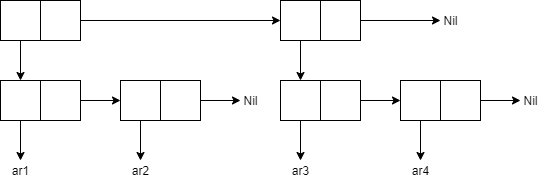
\includegraphics[scale=0.8]{1}
	\centering\caption{((ar1 ar2)(ar3 ar4))}
\end{figure}
\clearpage
\newpage
2) Написать функцию (f ar1 ar2), возвращающую: ((ar1)(ar2))
\begin{lstlisting}
	(defun f(ar1 ar2)
		(list
				(list ar1)
				(list ar2)
		)
	)
\end{lstlisting}
\begin{figure}[h!]
	\centering 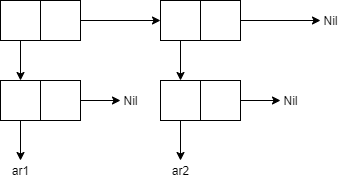
\includegraphics[scale=1]{2}
	\centering\caption{((ar1)(ar2))}
\end{figure}

3) Написать функцию (f ar1), возвращающую: (((ar1)))
\begin{lstlisting}
	(defun f(ar1 ar2)
		(list
				(list 
						(list ar1)
				)
		)
	)
\end{lstlisting}
\clearpage
\newpage
\begin{figure}[h!]
	\centering 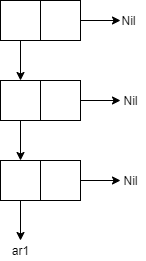
\includegraphics[scale=1]{3}
	\centering\caption{(((ar1)))}
\end{figure}

\section*{Ответы на вопросы:}
\addcontentsline{toc}{section}{Ответы на вопросы}
\textbf{1) Элементы языка:}
	\\ Атомами являются:
\begin{enumerate}
	\item \textbf{символы(идентификаторы)} - синтаксически - набор литер(букв латинского алфавита и цифр), начинающихся с буквы;
	\item \textbf{специальные символы - {T, Nil}} - используются для обозначения <<логических констант>>;
	\item \textbf{самоопределимые атомы} - натуральные числа, дробные числа, вещественные числа, строки - последовательность символов, заключенных в двойные апострофы.
\end{enumerate}
\hspace*{5mm} Более сложные данные в Lisp выстраиваются с помощью \textit{бинарных узлов}, содержащих пару указателей.
\\ \hspace*{5mm} \textbf{Точечная пара} – структура данных, состоящая из двух символьных выражений, разделенных точкой.
\\ \hspace*{5mm} \textbf{Список} – это структура данных. Может быть пустой и непустой. Если непустой,
то состоит из двух элементов: первый - любой формы, а второй - список. Список - это частный случай S-выражения.\cite{com}

\hspace*{-5mm} \textbf{2) Синтаксис элемента языка и их представление в памяти:}
\\ \hspace*{5mm} Синтаксически любая структура (точечная пара или список) заключается в круглые скобки ( A . B ) - точечная пара, ( А ) - список из одного элемента, пустой список изображается как Nil или (). Не пустой список по определению может быть изображен как ( A.(B.(C.(D())))), допустимо изображение списка последовательностью атомов, разделенных пробелами - (A B C D). Элементы списка могут, в свою очередь, быть списками (любой список заключается в круглые скобки), например - (A (B C) (D (E))). Таким образом, синтаксически наличие скобок является признаком структуры - списка или точечной пары. 
\\ \hspace*{5mm} Любая непустая структура Lisp в памяти представляется списковой ячейкой, хранящей два указателя на голову (первый элемент) и хвост - все остальные. 
\\ \textbf{3) Как воспринимается <<'>> ?}
\\ \hspace*{5mm} Употребление апострофа на жаргоне называется <<Квонтирование>>. Оно используется в случае, когда требуется заблокировать вычисление значения, иначе будет попытка вычислить значение. В самоопределяющих атомах, <<квантирование>> не требуется. Встроенной функцией заменяющее <<'>> - является функция <<quote>>.

\clearpage
\newpage
\printbibliography
\addcontentsline{toc}{section}{Список литературы}

\end{document}